\chapter{Rumor Analysis}

	\section{Combining Overlapping Clusters}	
	
	The earlier results show that increasing data to produce more as well as bigger clusters has a drawback since the time required to process such data increases proportionally with the number of days for which data is taken and thus is not scalable.If we need to see if any rumor is active from last 'n' days, we need to process the 'n' day's data plus the current day's data.Clearly this approach is not scalable as it requires re-computation of the last 'n' days data.An efficient way to do this is store the result for last 'n' days and combine it with the current day's data.By this technique,the unit of data that should be processed can be kept to one day.This each one day's processed data can be combined with earlier data to accurately represent the cluster.
	\\  
	\par 
	The earlier algorithm clusters tweets into candidate rumor clusters for each day to expedite the processing on the Hadoop cluster.But this may lead to disjoint clusters created for each day,where rumors may spread over multiple days.Such rumor clusters which are divided into separate clusters over multiple days must be combined into single cluster so that we can accurately model the cluster for it's temporal and quantitative  characteristics.Such a framework also allows us to add newer data  to existing clusters and check if any of the older rumors still exist or whether they have ceased.
	\\
	\par
	To enable faster processing of clusters,we process only the signal tweets as they form a small portion of the overall tweet volume.Jaccard distance is used to calculate the distance between two tweets.Prior to clustering the tweets, the tweet data is processed using standard text preprocessing techniques so that the clustering performance is not impacted due to noise in the text data.The tweets are then clustered using hierarchical clustering.Average linking method is used to cluster the tweets is due it's advantages over the other methods.Average-link clustering is a compromise between the sensitivity of complete-link clustering to outliers and the tendency of single-link clustering to form long chains that do not correspond to the intuitive notion of clusters as compact, spherical objects.Average-link clustering merges in each iteration the pair of clusters with the highest cohesion.
	\\
	\par
	The dendogram is cut at height 0.75 which is empirically the best value among all other values at which cut is done.Such a clustering will still lead to large number of small clusters.This is primarily due to the sparsity of the words contained in the tweets and the 140 character limit of each tweet.But these small clusters are indeed disjoint components of a bigger cluster.The algorithm 1 produces a list of clusters along with its summary features.These summary features can be used as semantic features to combine the clusters.For example, if a cluster obtained using the algorithm 2 contains summary features as f1,f2..fn, we can search other clusters where tweet has summary feature f1,f2,..fn.If such a tweet is found in another cluster of algorithm 1,the tweet and all other tweets containing in it's cluster are combined with the original cluster.This process is carried out transitively until no cluster produced by algorithm 1 can be further merged into a cluster produced by algorithm 2.	
	\\
	\par
	The entire algorithm is outlined below.
	
	\begin{algorithm}[H]
		\caption{{\em Tweet clustering algorithm - Multiple days}}
		\textbf{Input:} Signal tweets with summary features  from output produced by Algorithm 1 \\
		Non Signal tweets with summary features  from output produced by Algorithm 1 \\
		\textbf{Output:} Clusters of candidate rumors spanning multiple days \\ 
		\begin{minipage}{\linewidth}
			\begin{algorithmic}[1]	 	
				\FOR {All tweets in input-signal-tweets}
				\STATE Remove punctuation from the tweet
				\STATE Remove all the extra white space between words
				\STATE Convert all the words in tweet to lowercase
				\STATE Remove stopwords from the tweet	
				\ENDFOR
				
				\FOR {Tweet 'a' in input-signal-tweets}
				\FOR {Tweet 'b' in input-signal-tweets}
				\STATE Calculate word-level Jaccard between tweet 'a' and tweet 'b' and store the result in the distance matrix at location distance[a][b]
				\ENDFOR
				\ENDFOR
				
				\STATE Use hierarchical clustering using average linkage to produce the dendogram using the distance matrix
				\STATE Cut the dendogram at height determined empirically to determine the clusters
				\STATE Rank the clusters based on decreasing order of their size
				\FOR{ Each cluster 'c2' produced by algorithm 2}
				\STATE Extract unique summary features contained in the cluster
				\IF { A tweet in cluster 'c1' produced by algorithm 1 contains these summary features }
				\STATE Combine cluster 'c1' with 'c2'
				\ENDIF
				\STATE Repeat above steps until no cluster 'c1' can be further merged into cluster 'c2'
				
				\FOR{All input-non-signal-tweets}
				\IF { tweet summary matches to any unique summary features contained in the cluster }
				\STATE Add non-signal tweet to cluster
				\ENDIF	   
				\ENDFOR
				\ENDFOR
			\end{algorithmic}
		\end{minipage}
	\end{algorithm}
	
			 
	\section{Results - Clustering }
	 \begin{figure}[H]
	 	\centering
	 	\begin{minipage}{.7\linewidth}
	 		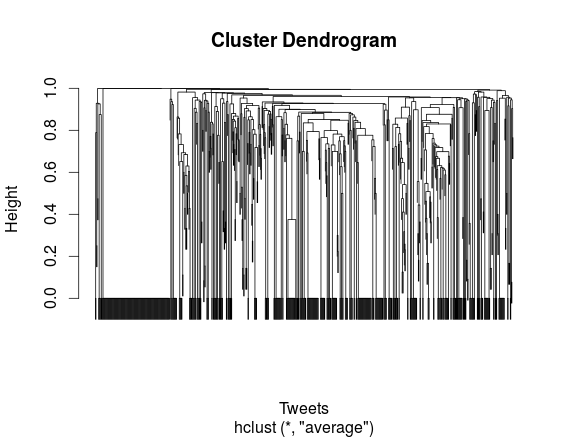
\includegraphics[width=\linewidth]{images/dendogram.png}
	 		\captionof{figure}{Cluster Dendrogram}
	 		\label{img5}
	 	\end{minipage}
	 \end{figure} 	
	 
	 \begin{figure}[H]
	 	\centering
	 	\begin{minipage}{.7\linewidth}
	 		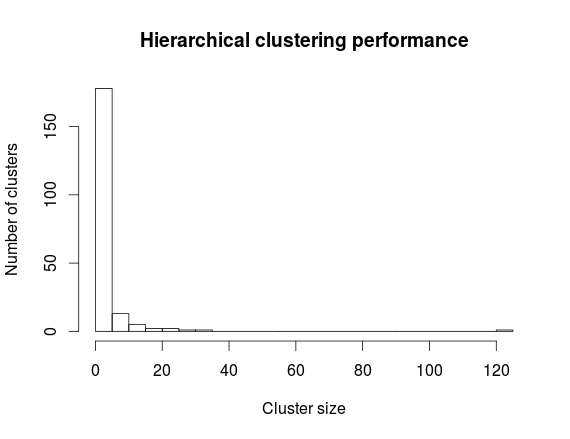
\includegraphics[width=\linewidth]{images/size_of_clusters.png}
	 		\captionof{figure}{Cluster size histogram}
	 		\label{img6}
	 	\end{minipage}
	 \end{figure} 	
	 
	 
	 Figure \ref{img5} shows the dendogram using hierarchical clustering of signal tweets using word level Jaccard distance.When this tree is cut at height 0.75, we get the clusters along with their size as shown in figure \ref{img6}.The histogram shows that we have a very large number of small clusters and a very small number of large clusters.Therefore, we need to combine these clusters into larger ones using the common semantic features that were obtained from algorithm 1.
	 
	 \section {Temporal analysis}
	 The next step involves the classification of the rumor clusters as rumor/non-rumors.The first focus is on the temporal aspects of the cluster.Other quantitative properties of the rumor will be explored later.We examine the rate of growth of tweet volume in a tweet cluster as a feature to classify the cluster.To calculate the rate of growth,the tweets are first sorted according to their tweet date.A new attribute rank 'i' is added to each tweet indicating that it is the 'i'th ranked tweet in the cluster according to its create date.A plot of tweet created date vs the rank of tweet in the cluster helps to determine the rate of growth of the tweet volume in the cluster.Analyzing the slope of distinct segments in the plot of can help to distinguish between rumor /non rumor.Each rumor cluster may have different size,hence we perform min-max normalization on the rank attribute to restrict it's values between 0-1 for any range of data.The min-max normalization is carried out as follows,where \begin{equation} x=(x_1,...,x_n) \end{equation} and z is now the ith normalized data :-
	 
	 \begin{equation}
	 z_i=\frac{x_i-\min(x)}{\max(x)-\min(x)}
	 \end{equation}

 \section{Results - Temporal Analysis }
 
 \begin{figure}[H]
	\centering
	\begin{minipage}{.45\linewidth}
		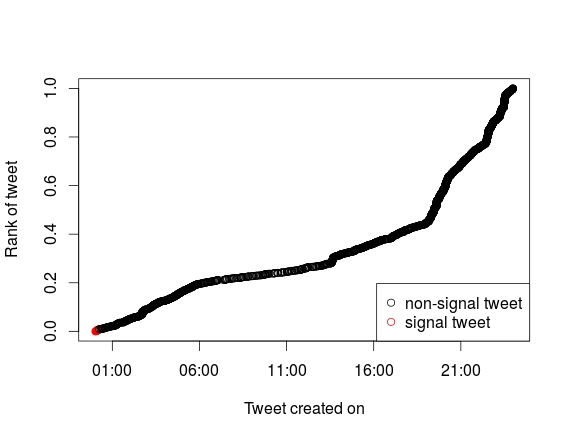
\includegraphics[width=\linewidth]{images/nrumor1.jpeg}
		\captionof{figure}{Tweet Date vs Rank of Tweet - Example 1}
		\label{nr1}
	\end{minipage}
	\hspace{.05\linewidth}
	\begin{minipage}{.45\linewidth}
		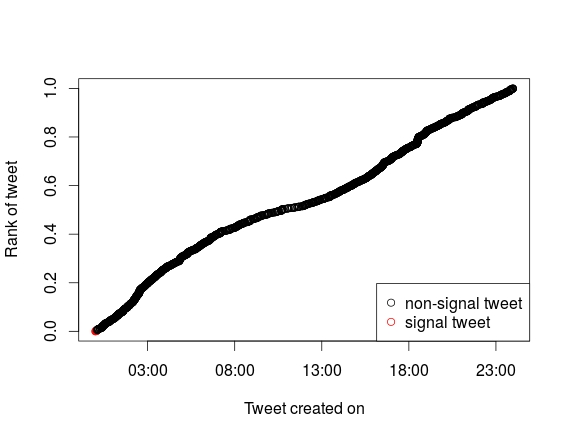
\includegraphics[width=\linewidth]{images/nrumor2.jpeg}
		\captionof{figure}{Tweet Date vs Rank of Tweet - Example 2}
		\label{nr2}
	\end{minipage}
	\centering
	\begin{minipage}{.45\linewidth}
		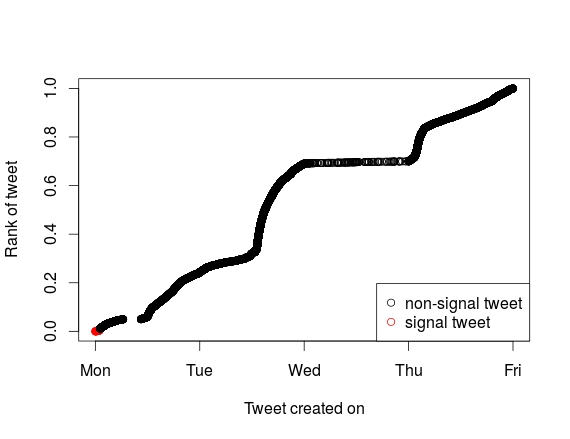
\includegraphics[width=\linewidth]{images/nrumor3.jpeg}
		\captionof{figure}{Tweet Date vs Rank of Tweet - Example 3}
		\label{nr3}
	\end{minipage}
	\hspace{.05\linewidth}
	\begin{minipage}{.45\linewidth}
		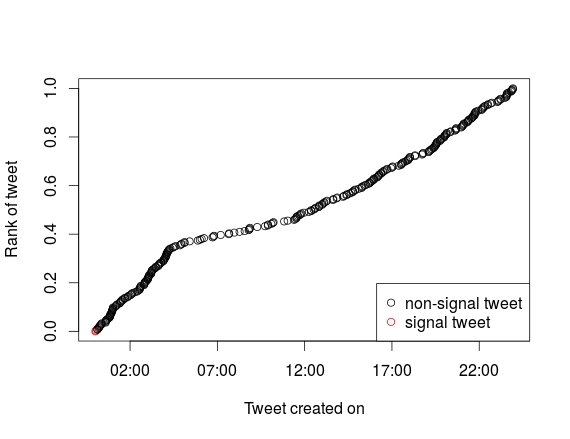
\includegraphics[width=\linewidth]{images/nrumor4.jpeg}
		\captionof{figure}{Tweet Date vs Rank of Tweet - Example 4}
		\label{nr4}
	\end{minipage}
\end{figure}

  In Figure \ref{nr1} we plot the time of tweet v/s the rank of the tweet(i.e. sequence number of the tweet when ordered according to it's create time).
  We can say that the growth of a non-rumor is fairly constant throughout it's lifetime.Since inception till it's end,the number of people posting about it does not deviate much.This can be seen by absence of sparse dots on the plot(we see this pattern in rumor when it's starts to fade away).Due to such behavior,this plot is a non-sparse curve.Owing to less number of distinct segments than a rumor plot,we can fit a linear line through a non-rumor cluster plot with less sum-of-square error than a rumor plot.Figure \ref{nr2},\ref{nr3} and \ref{nr4} show another similar instance of a clusters which do not constitute a rumor. 

 
 
\begin{figure}[H]
	\centering
	\begin{minipage}{.45\linewidth}
		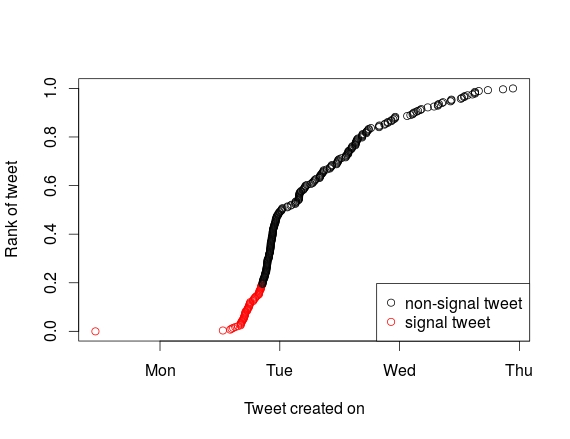
\includegraphics[width=\linewidth]{images/rumor1.jpeg}
		\captionof{figure}{Tweet Date vs Rank of Tweet - Example 1}
		\label{r1}
	\end{minipage}
	\hspace{.05\linewidth}
	\begin{minipage}{.45\linewidth}
		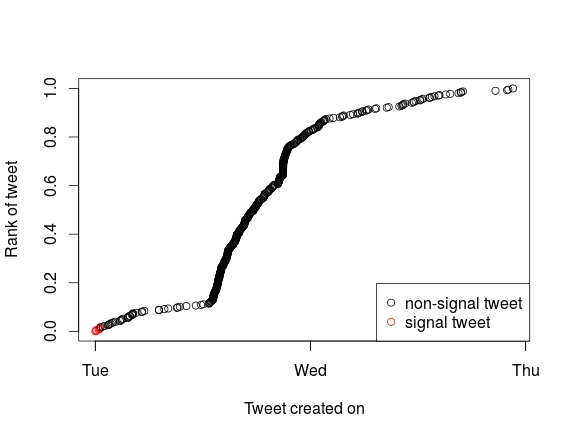
\includegraphics[width=\linewidth]{images/rumor2.jpeg}
		\captionof{figure}{Tweet Date vs Rank of Tweet - Example 2}
		\label{r2}
	\end{minipage}
	\centering
	\begin{minipage}{.45\linewidth}
		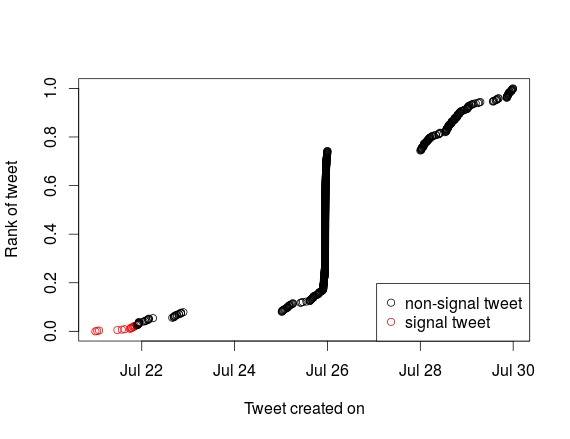
\includegraphics[width=\linewidth]{images/rumor3.jpeg}
		\captionof{figure}{Tweet Date vs Rank of Tweet - Example 3}
		\label{r3}
	\end{minipage}
	\hspace{.05\linewidth}
	\begin{minipage}{.45\linewidth}
		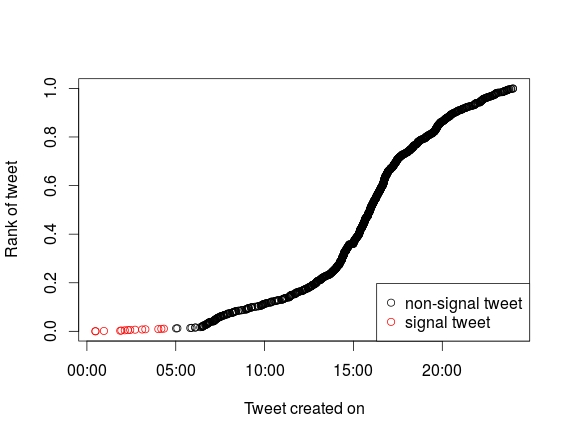
\includegraphics[width=\linewidth]{images/rumor4.jpeg}
		\captionof{figure}{Tweet Date vs Rank of Tweet - Example 4}
		\label{r4}
	\end{minipage}
\end{figure}



 
  In Figure \ref{r1} we plot the time of tweet v/s the rank of the tweet(i.e. sequence number of the tweet when ordered according to it's create time).It shows that the growth of a rumor is non-linear.We find different phases where the rumor starts to spread,then increases at a rapid rate and ultimately decaying after a certain point in time.Figure \ref{r2},\ref{r3} and \ref{r4} shows another similar instance of rumor growth rate.These different stages can be found by estimating the number of segments that are required to plot the curve.A rumor has many stages where rate of growth will be different at each stage thereby each of them resulting in a distinct segment on the plot.
 

 \section{Results - Burst Analysis }
 
 We now show the difference in burst patterns that are visible in rumors and non rumors.Here we divide the tweets in a rumor clusters in 30 bins divided by equal time intervals and plot the frequency of tweets in the corresponding bins.
 
 \begin{figure}[H]
 	\centering
 	\begin{minipage}{.45\linewidth}
 		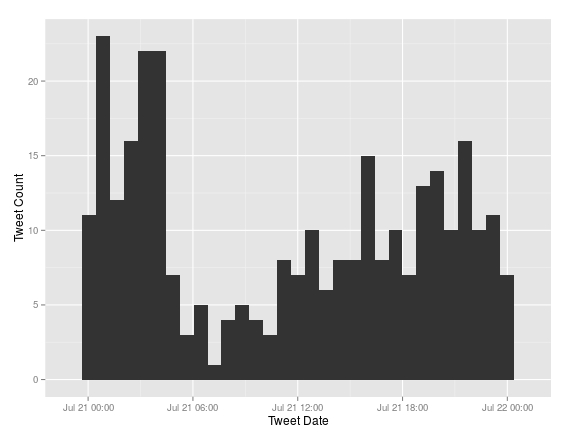
\includegraphics[width=\linewidth]{images/nrumorburst1.jpeg}
 		\captionof{figure}{Tweet Date vs Frequency - Example 1}
 		\label{nrb1}
 	\end{minipage}
 	\hspace{.05\linewidth}
 	\begin{minipage}{.45\linewidth}
 		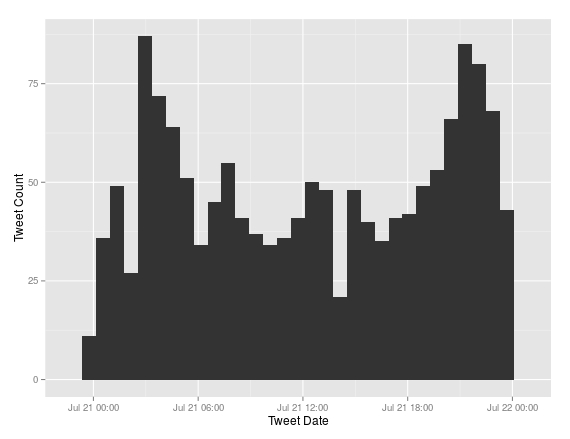
\includegraphics[width=\linewidth]{images/nrumorburst2.jpeg}
 		\captionof{figure}{Tweet Date vs Frequency - Example 2}
 		\label{nrb2}
 	\end{minipage}
 \end{figure}
 
  Figures \ref{nrb1} and \ref{nrb2} show the pattern observed in tweets which are non rumors.The distribution shows that number of tweets in every bin does not differ much.There is no presence of spikes in the plot which dominate every other bin in the plot.
 
  \begin{figure}[H]
  	\centering
  	\begin{minipage}{.45\linewidth}
  		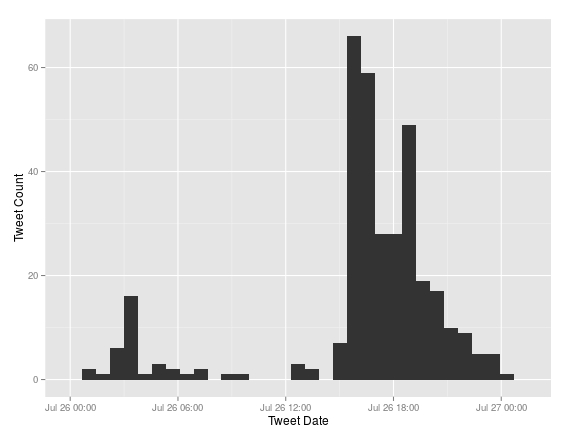
\includegraphics[width=\linewidth]{images/rumorburst1.jpeg}
  		\captionof{figure}{Tweet Date vs Frequency - Example 1}
  		\label{rb1}
  	\end{minipage}
  	\hspace{.05\linewidth}
  	\begin{minipage}{.45\linewidth}
  		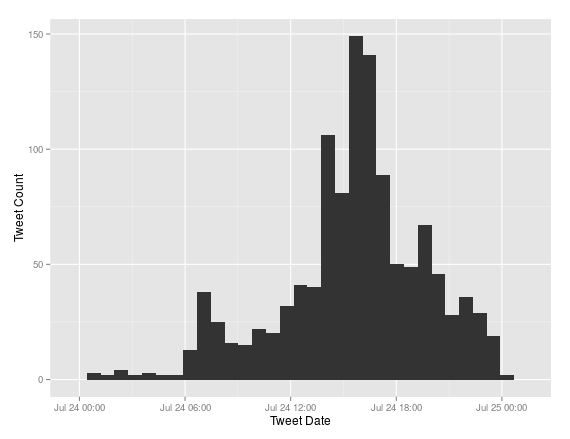
\includegraphics[width=\linewidth]{images/rumorburst3.jpeg}
  		\captionof{figure}{Tweet Date vs Frequency - Example 2}
  		\label{rb2}
  	\end{minipage}
  \end{figure}	
  
   Figures \ref{rb1} and \ref{rb2} show the pattern observed in tweets which are rumors.The distribution shows that number of tweets in every bin differs by a significant quantity.There exists at least one significant spike in the plot towards end of the plot when the rumor starts to become viral.Also,the initial bins seems to be less frequent as the rumor has still not propagated through a large number of users.
  	

\section{Results - Data Analysis }

  The following figures \ref{nrd1} and \ref{nrd2} show the Tweet Date vs Tweet Is-Signal scatter plot.We plot these values for all combinations of values of number of user mentions and number of hashtags thus resulting in several sub plots.
  The Tweet-Is-Signal property can have a value of 1 or 0 depending on whether the tweet contains enquiry patterns.
 
\begin{figure}[H]
	\centering
	\begin{minipage}{.7\linewidth}
		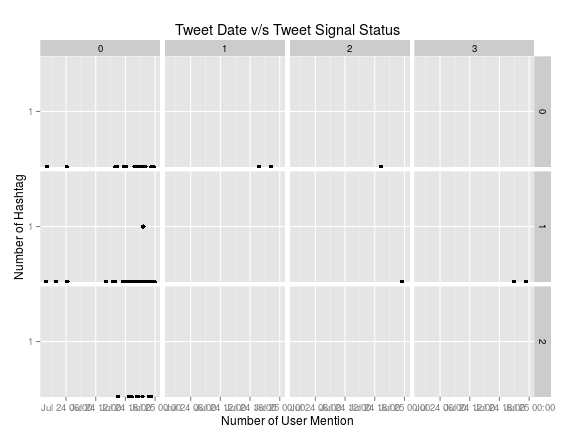
\includegraphics[width=\linewidth]{images/qp_nrumor1.jpeg}
		\captionof{figure}{Tweet Date vs Tweet-Is-Signal}
		\label{nrd1}
	\end{minipage}
\end{figure}

\begin{figure}[H]	
	\centering
	\begin{minipage}{.7\linewidth}
		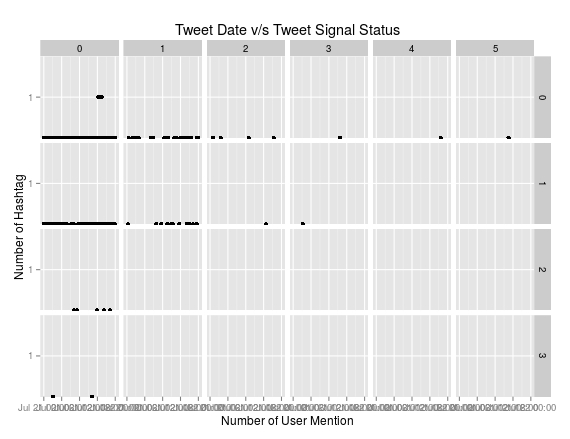
\includegraphics[width=\linewidth]{images/qp_nrumor2.jpeg}
		\captionof{figure}{Tweet Date vs Tweet-Is-Signal}
		\label{nrd2}
	\end{minipage}
\end{figure}

 Figures \ref{nrd1} and \ref{nrd2} show the behavior observed in tweet clusters that are non rumors.We see that signal tweets in such a case do not contain usermentions as well as hashtags except barring a few exceptions.

\begin{figure}[H]
	\centering
	\begin{minipage}{.7\linewidth}
		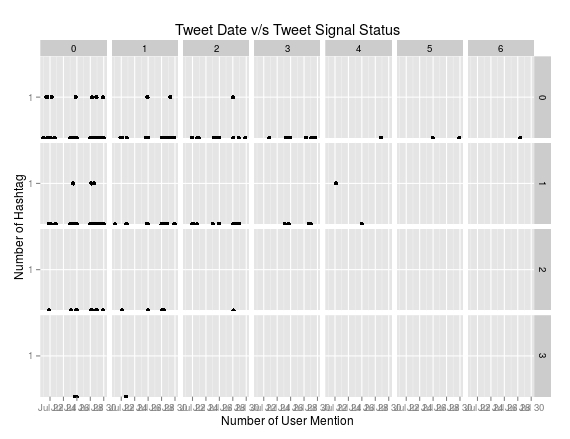
\includegraphics[width=\linewidth]{images/qp_rumor1.jpeg}
		\captionof{figure}{Tweet Date vs Tweet-Is-Signal}
		\label{rd1}
	\end{minipage}
\end{figure}
	
\begin{figure}[H]
	\centering
	\begin{minipage}{.7\linewidth}
		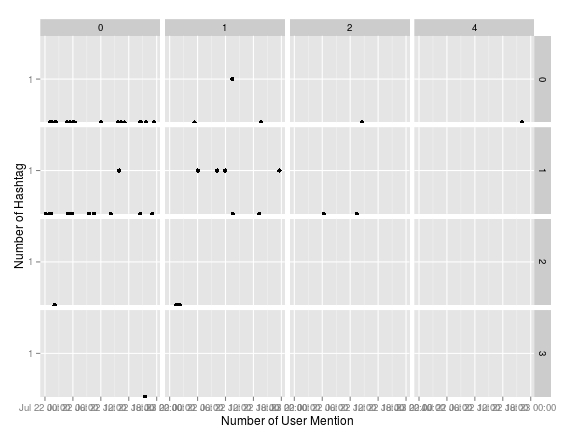
\includegraphics[width=\linewidth]{images/qp_rumor2.jpeg}
		\captionof{figure}{Tweet Date vs Tweet-Is-Signal}
		\label{rd2}
	\end{minipage}
\end{figure}

 Figures \ref{rd1} and \ref{rd2} show the behavior observed in tweet clusters that are rumors.We see that signal tweets in such a case  at least one contain user mentions or hashtags or a combination of both.
 
 \section{Summary}
 
 This chapter has focused on tweet clustering to accurately gather all tweets related to rumor.The dendrogram after initial clustering showed that clusters are not formed accurately due to sparse words in tweets and these clusters need to be combined further using another clustering algorithm.This helps in better prediction towards decision in the analysis part.The analysis part covered the difference in temporal and non-temporal properties of rumors which helps us to distinguish the both of them accurately.  	